\newpage
\begin{center}\large Addendum: CPU API-v2 capacity refusals\end{center}
\textbf{Two actual requests, no allocation or scientific trial.} Fresh
\path{resource-runs/cpu-api-v2-01}, observed approximately 06:03:31--06:03:35 UTC,
is bound to published controller source
\texttt{493f0ca1b7183dbd9e42ddcf8c44c650754e3fdb}. Both exact CPU-create
requests returned HTTP400 with the explicit provider message: ``There are no
longer any instances available with the requested specifications.''

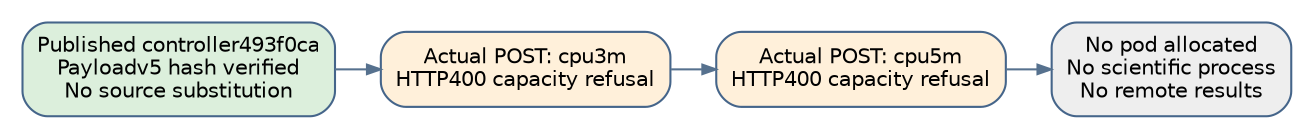
\includegraphics[width=\linewidth]{cpu-api-v2-flow.png}

\begin{center}
\begin{tabular}{llll}
\toprule
Request & Catalog-derived RAM & Catalog availability & Actual response\\
\midrule
cpu3m,32 vCPU &256 GB &HIGH &HTTP400 capacity refusal\\
cpu5m,32 vCPU &256 GB &LOW &HTTP400 capacity refusal\\
\bottomrule
\end{tabular}
\end{center}
Catalog quotes were \$1.76/hour and \$2.08/hour. These are request/catalog
metadata, not measurements of a 256 GB instance or of research performance.
The controller stopped after the two explicit refusals, without allocating
another pod, starting science or fetching remote results. Refusal does not
establish general lack of capacity, mathematical failure or security.

\textbf{Source and raw evidence.} Redacted requests, both refusal records,
catalog, ownership intent, controller stdout/stderr and original outcome are
retained under the fresh resource directory and adjacent controller logs.
Public-source proof records an unauthenticated fetch of 1,626,771 bytes and
the unchanged payloadv5 hash prefix \texttt{e269ad82ff1ff772}; the full digest
and source URL are retained in \path{public-source-proof.json} under that
directory. This binds public delivery provenance, not a scientific execution.
The outcome retains pod id null and results fetched false.

\textbf{Independent no-allocation closeout.} Root's separate receipt records a
complete API-v2 inventory (one page), zero exact-request matches and zero
active campaign resources. No provider DELETE was required. Root verified the
exact local watchdog process identity/owner, stopped only that process with
SIGTERM and recorded it stopped. The original controller outcome's false
absence/deleted fields remain unchanged; the separate closeout binds the
no-allocation observation. Receipt:
\path{resource-runs/cpu-api-v2-01/root-no-allocation-closeout.json}.

The frozen intent watchdog could otherwise poll an empty inventory every two
seconds until its deadline. Explicit closeout avoids those needless local
polls; controller/scientific sources were not changed.


\textbf{Evidence boundary.} This attempt supplied no closure output, D,
curve computation, throughput, relation yield or challenge progress. Run1's
GPU control, original ingestion refusal, separate local correction and
censored closure remain unchanged; GPU-v3 is a separate failed-host record.
Historical campaign rates, forecasts and scientific status remain unchanged.
The previous four-page report is preserved as \path{reports/gpu-v3-report.pdf},
SHA256 prefix \texttt{fb389bfbcf60bc1f}. Full source-linked record:
\texttt{CPU\_API\_V2\_RESULTS.md}.
